\chapter{Similar applications}

Neural Network Models as well as Machine Learning algorithms provide various versatile and adaptive methods for non-linear problem solving. Because of these reasons , there are numerous applications which perform the task of musical/audio classification using the aforementioned techniques. We will discuss in the following sections about three of those applications.

\section{Spektrum}

Spektrum is a multi-platform music genre classificator and music recommandation system developed in the context of the course "Application Challenges for
Machine Learning on the example of IBM Power AI", by the team consisting of Marte Vinje, Moritz Klimmek, Thomas Salzer, Aaron Hümmecke, Lukas Vorwerk \cite{spektrum} . The application consists of two parts:
\begin{itemize}
	\item Music Genre Classification: Performed by a Convolutional Neural Network Model which analyzes the MEL spectogram of a given input song.
	\item Music Recomandation: Generating suggestions by making use of a combination collaborative filtering
		and content based filtering.
\end{itemize}

\begin{figure}[H]
	\centering
	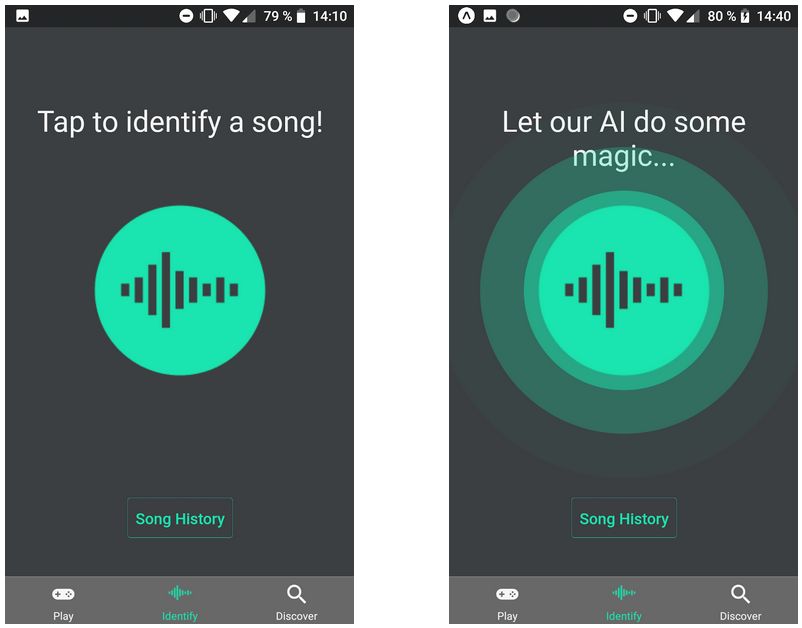
\includegraphics{images/spektrum.png}
	\caption{Interfata Spektrum}
\label{ANN}
\end{figure}


\section{Titlul secțiunii 2}

Pellentesque pulvinar pellentesque habitant morbi tristique senectus et. Ornare suspendisse sed nisi lacus sed viverra tellus in hac. Non sodales neque sodales ut etiam sit. In hendrerit gravida rutrum quisque non. Diam quam nulla porttitor massa id neque aliquam. Diam sit amet nisl suscipit adipiscing bibendum est ultricies integer. Cras fermentum odio eu feugiat pretium nibh ipsum. Egestas integer eget aliquet nibh praesent tristique magna. Porttitor eget dolor morbi non arcu risus quis varius quam. Gravida rutrum quisque non tellus orci. Diam volutpat commodo sed egestas egeas.
